\newpage
\section{Auswertung}
\label{sec:Auswertung}

\subsection{Untergrund}
\label{sec:Untergrund}
Die Messwerte füe beide Heizraten sind in Abbildung \ref{fig:1} abgebildet. 
Dabei sind die gemessenen Ströme in pA gegen die Temperatur der Probe in K aufgetragen.
Der Untergrund wird durch eine Exponentialfunktion der Form,

\begin{equation}
    f(x) = a \cdot \text{exp} \left( \frac{-b}{T} \right) + c,
\end{equation}
an das zweite Maximum gefittet.
Daraus ergeben sich die Parameter: 

\begin{align*}
    &\text{Messung 1:}\\
    & a = 0.49 \pm 0.32 \,A    &&  b = 3634.88 \pm 187.06 \,K    &&  c = -2.38 \pm 0.16 \cdot 10^{-9}\,A \\
    &\text{Messung 2:}\\
    & a = 0.09 \pm 0.04 \,A    &&  b = 3067.80 \pm 136.59 \,K    &&  c = -2.72 \pm 0.23 \cdot 10^{-9}\,A \\
\end{align*}
Diese Fits sind ebenfalls in Abbildung \ref{fig:1} zu sehen.
Um das Signal mit reduziertem Untergrund zu erhalten, wird nun der gefittete Untergrund von den Messwerten subtrahiert.
Die Untergrund bereinigten Messwerte sind in Abbildung \ref{fig:2} dargestellt.

\begin{figure}
    \centering
    \begin{subfigure}[b]{0.49\textwidth}
        \centering
        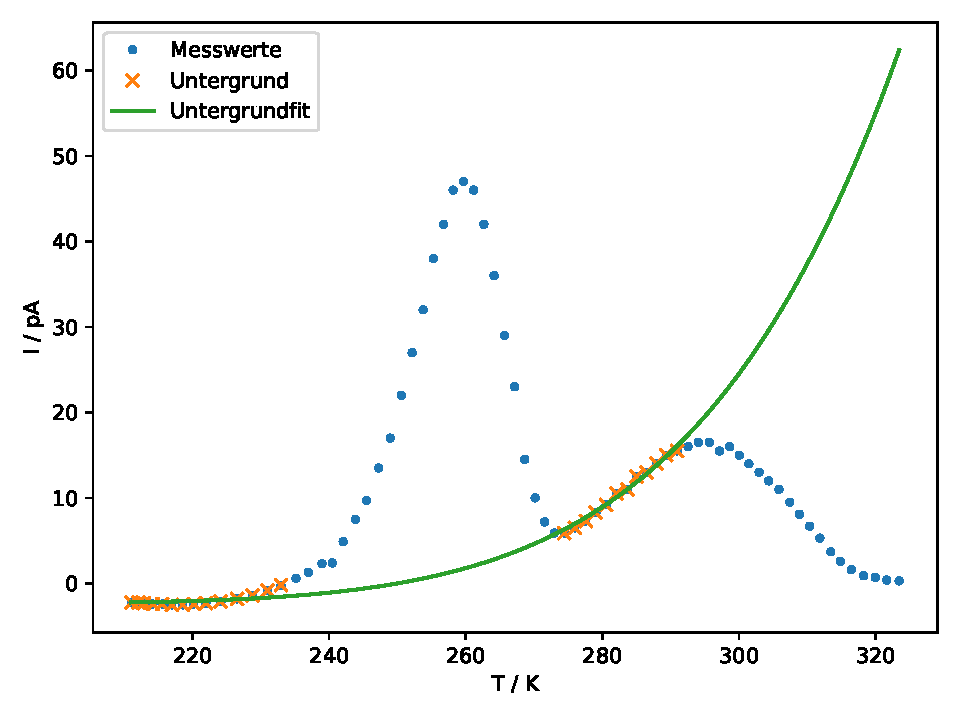
\includegraphics[width= \textwidth]{plots/mitunter_1.5grad.pdf}
    \end{subfigure}
    \hfill
    \begin{subfigure}[b]{0.49\textwidth}
        \centering
        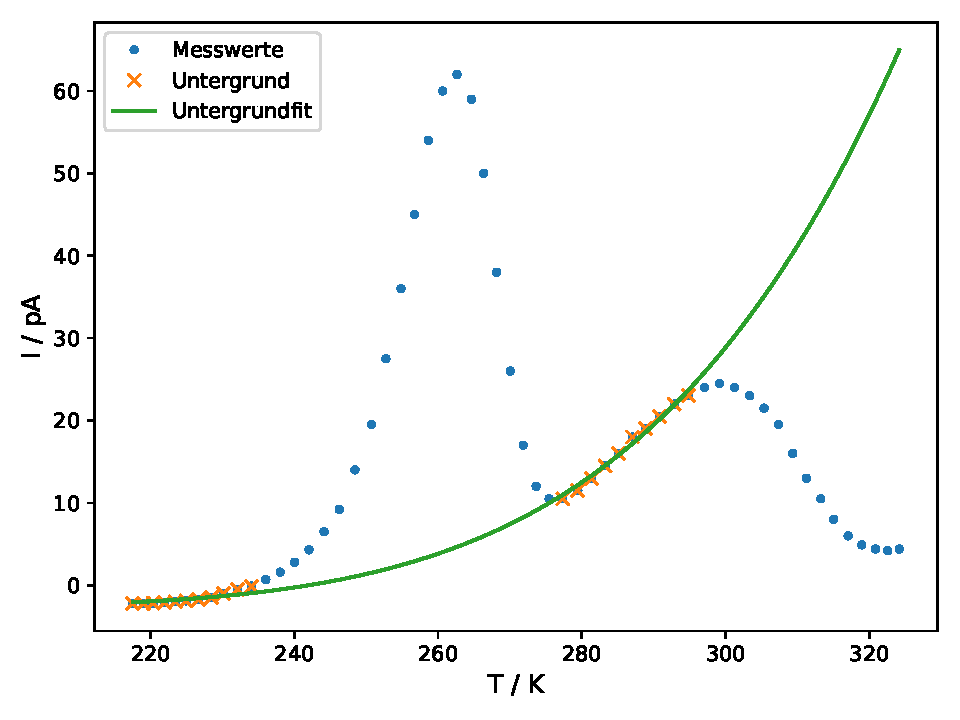
\includegraphics[width= \textwidth]{plots/mitunter_2grad.pdf}
    \end{subfigure}
    \caption{Die aufgenommenen Messwerte, so wie die gefittete Untergrundfunktion mit der form einer Exponentialfunktion, für Messung 1 (links) und Messung 2 (rechts).}
    \label{fig:1}
\end{figure}


\begin{figure}
    \centering
    \begin{subfigure}[b]{0.49\textwidth}
        \centering
        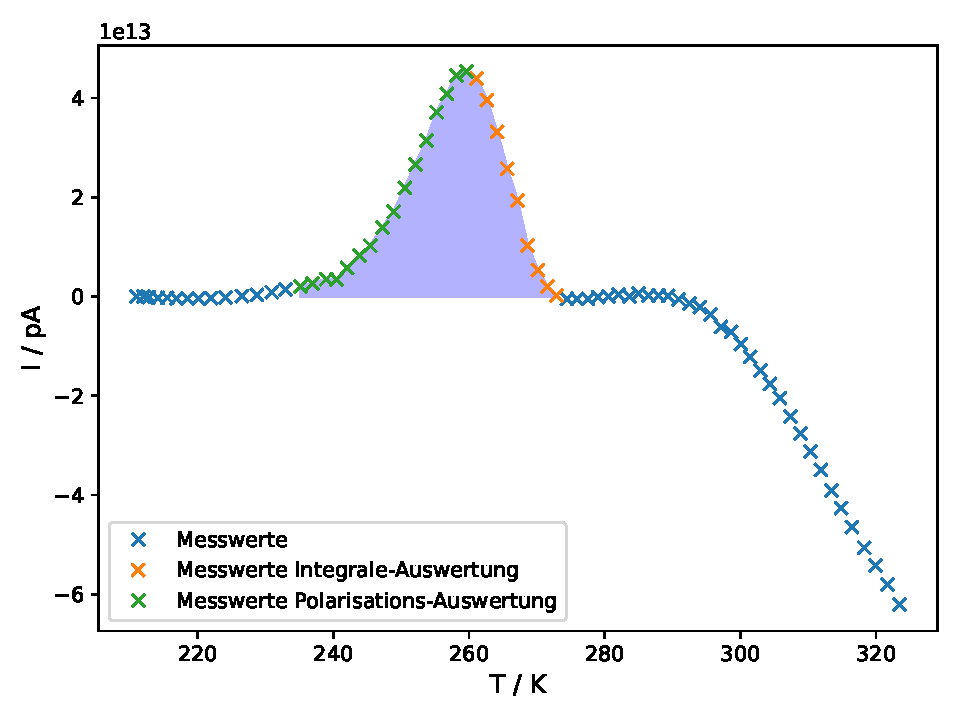
\includegraphics[width= \textwidth]{plots/ohneunter_1.5grad.pdf}
    \end{subfigure}
    \hfill
    \begin{subfigure}[b]{0.49\textwidth}
        \centering
        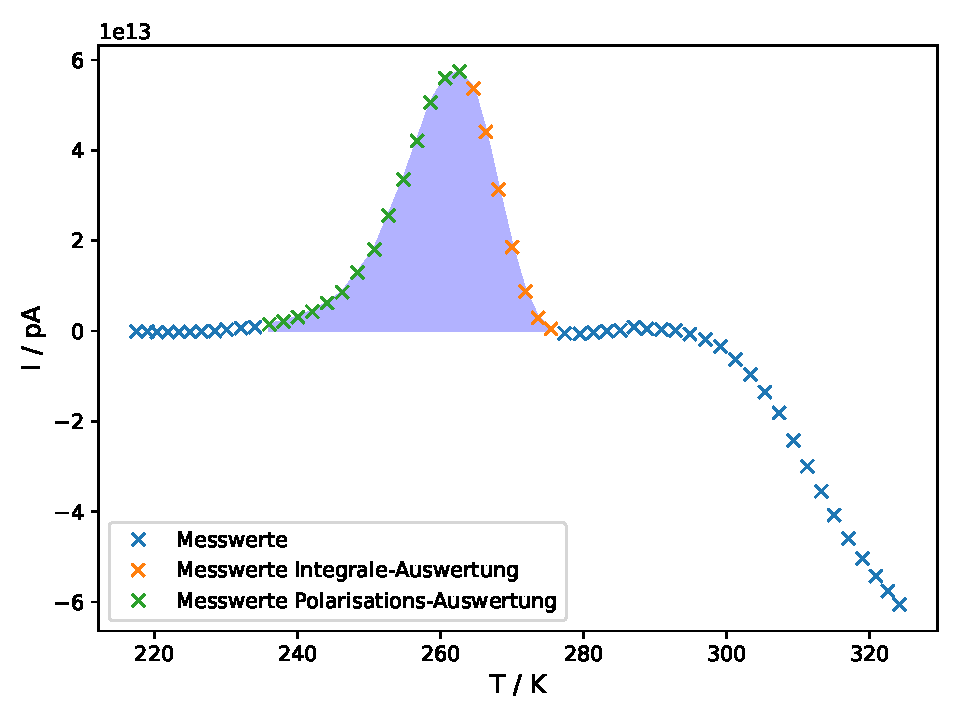
\includegraphics[width= \textwidth]{plots/ohneunter_2grad.pdf}
    \end{subfigure}
    \caption{Die Untergrund bereinigten Messwerte von Messung 1 (links) und Messung 2 (rechts).}
    \label{fig:2}
\end{figure}




\subsection{Heizrate}
\label{sec:Heizrate}

Bei den im Folgennden genutztenn Ansätze zur bestimmung der Aktiwierungsenergie W, wird angenommen, dass die Heizrate konstant ist.
Diese Heizrate wird durch Formel \ref{equ:A1} bestimmt.

\begin{equation}
    b = \frac{1}{n-1} \sum_{i=1}^{n} \frac{T_i - T_{i-1}}{\SI{1}{\minute}}
    \label{equ:A1}
\end{equation}
Für die erste Messreihe folgt eine Heizrate von $b_1 = 1.58 \pm 0.19 \,\frac{\text{K}}{\text{min}}$ und für die Zweite $b_2 = 1.90 \pm 0.25 \,\frac{\text{K}}{\text{min}}$.




\subsection{Aktivierungsenergie - Polarisationsansatz}
\label{sec:pol}

Für den Polarisationsansatz werden die Messwerte nach Formel \ref{equ:1} umgeformt. 
Es wird der Logarithmus des Depolarisationsstroms gebildet und gegen die inverse Temperatur abgebildet.
Anschließend wird eine Ausgleichsrechnung der Form 

\begin{equation}
    \text{ln} I(T) = m \cdot \frac{1}{T} + n
\end{equation}
durchgeführt.
Die ermittelten Werte sind:

\begin{align*}
    &\text{Messung 1:}\\
    & m = -10620.99 \pm 604.32 \,T    &&  n = 45.25 \pm 2.44   \\
    &\text{Messung 2:}\\
    & m = -10195.23 \pm 557.63 \,T    &&  n = 33.56 \pm 4.26   \\
\end{align*}
Die Ausgleichsgeraden sind in Abbildung \ref{fig:3} abgebildet.
Aus der Gleichung 
\begin{equation}
    W = -k_B \cdot m,
    \label{equ:A2}
\end{equation}
ergibt sich die Aktivierungsenergie zu

\begin{align*}
    &\text{Messung 1:}\\
    & W = 0.92 \pm 0.05 \,eV  \\
    &\text{Messung 2:}\\
    & W = 0.88 \pm 0.05 \,eV.  \\
\end{align*}

\begin{figure}
    \centering
    \begin{subfigure}[b]{0.49\textwidth}
        \centering
        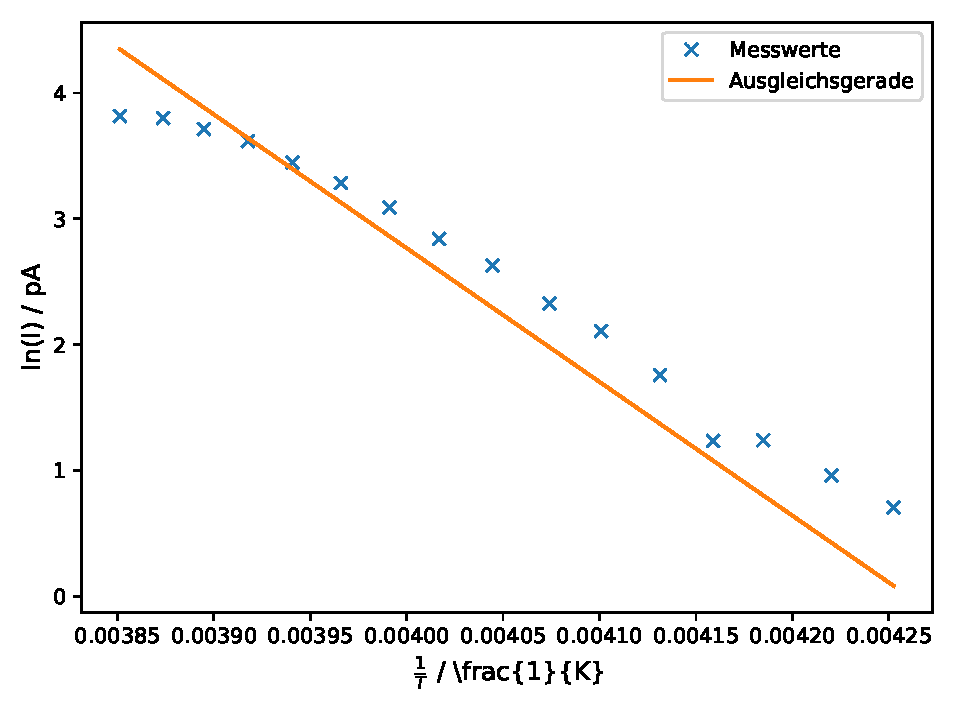
\includegraphics[width= \textwidth]{plots/asc_1.5grad.pdf}
    \end{subfigure}
    \hfill
    \begin{subfigure}[b]{0.49\textwidth}
        \centering
        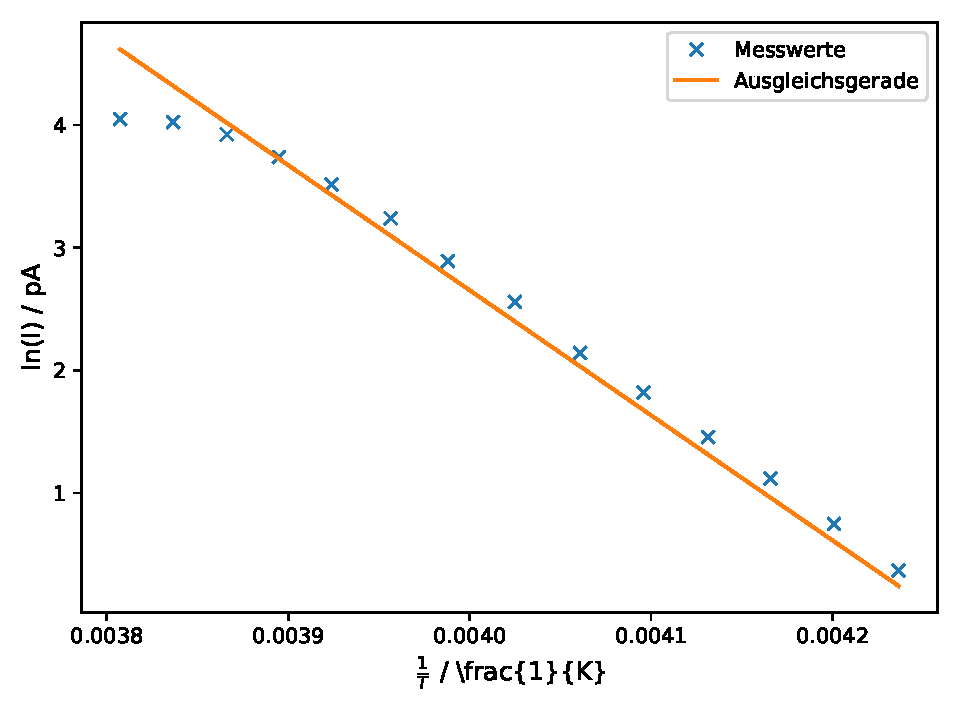
\includegraphics[width= \textwidth]{plots/asc_2grad.pdf}
    \end{subfigure}
    \caption{Messwerte des ersten Peak, so wie die Ausgleichsgerade des Polarisationsansatzes, für Messung 1 (links) und Messung 2 (rechts).}
    \label{fig:3}
\end{figure}




\subsection{Aktivierungsenergie - Integralansatz}
\label{sec:int}

Bei der Integralmethode wird nach Gleichung \ref{equ:2}, $\frac{1}{T}$ gegen $\text{ln} \left( \frac{\int_{T}^{\infty} I(T^{'}) \text{d}T^{'}}{b \tau_0 \cdot I(T)} \right)$ aufgetragen und eine lineare Ausgleichsrechnung der Formel

\begin{equation}
    y = m \cdot x + b
\end{equation}
durchgeführt.
Diese Ausgleichgeraden sind in Abbildung \ref{fig:4} zu finden.
Mit Hilfe von \ref{equ:A2} wird dir Aktivierungsenergie W berechnet.

\begin{align*}
    &\text{Messung 1:}\\
    & W = 0.72 \pm 0.10 \,eV \\
    &\text{Messung 2:}\\
    & W = 0.69 \pm 0.09 \,eV  \\
\end{align*}

\begin{figure}
    \centering
    \begin{subfigure}[b]{0.49\textwidth}
        \centering
        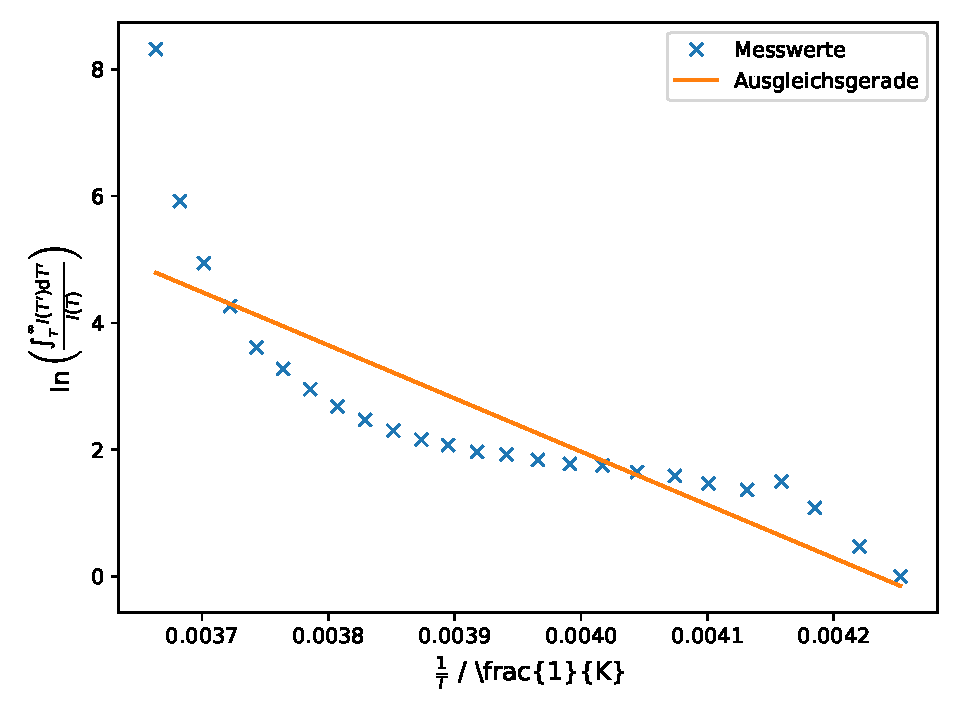
\includegraphics[width= \textwidth]{plots/int_1.5grad.pdf}
    \end{subfigure}
    \hfill
    \begin{subfigure}[b]{0.49\textwidth}
        \centering
        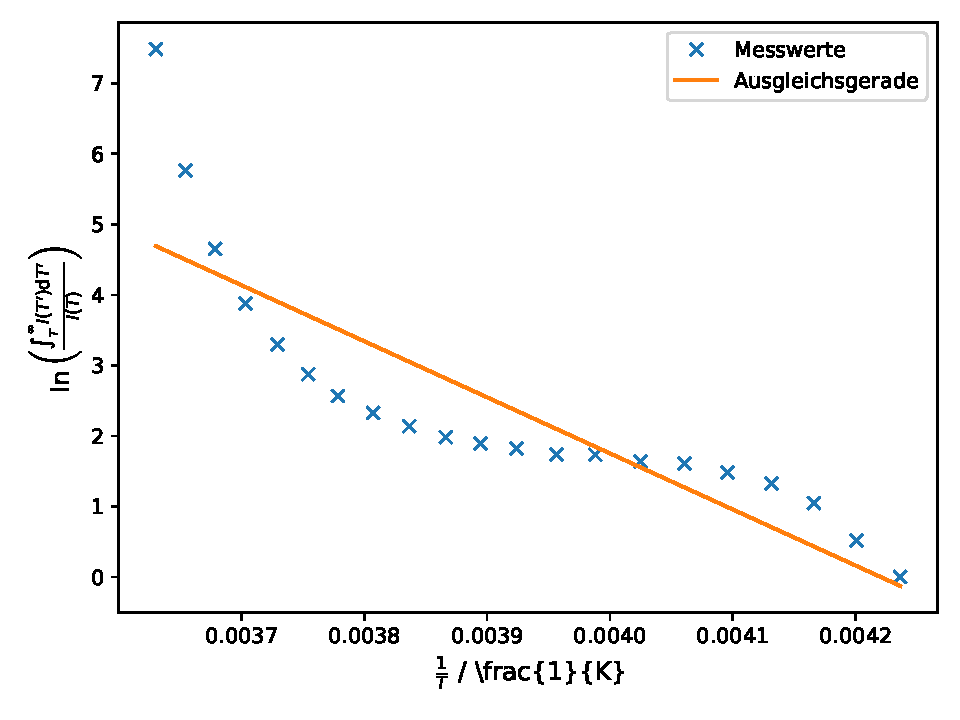
\includegraphics[width= \textwidth]{plots/int_2grad.pdf}
    \end{subfigure}
    \caption{Messwerte des ersten Peak, so wie die Ausgleichsgerade des Integralansatzes, für Messung 1 (links) und Messung 2 (rechts).}
    \label{fig:4}
\end{figure}






\subsection{Relaxationszeit}
\label{sec:rel}
Mit den konstanten Heizraten und Aktivierungsenergien kann nach Gleichung \ref{equ:3} die Relaxationszeit berechnet werden.
Für die durch den Polarisationsansatz bestimmten Aktivierungsenergien ergeben sich die folgenden Relaxationszeiten: 

\begin{align*}
    &\text{Messung 1:}\\
    & \tau = (4 \pm 10) \cdot 10^{-16} \,s    \\
    &\text{Messung 2:}\\
    & \tau = (3 \pm 0.65) \cdot 10^{-16} \,s  \\
\end{align*}
Mit den Temperaturen des maximalen Depolarisationsstromes $T_{max,1} = 259.65 \,K $ und $T_{max,2} = 262.65 \,K $.
Für die durch den Integralansatz berechneten Aktivierungsenergien folgt:

\begin{align*}
    &\text{Messung 1:}\\
    & \tau = (2.82 \pm 12.62) \cdot 10^{-12} \,s    \\
    &\text{Messung 2:}\\
    & \tau = (19.45 \pm 83.32) \cdot 10^{-12} \,s  \\
\end{align*}


%\begin{figure}
%    \centering
%    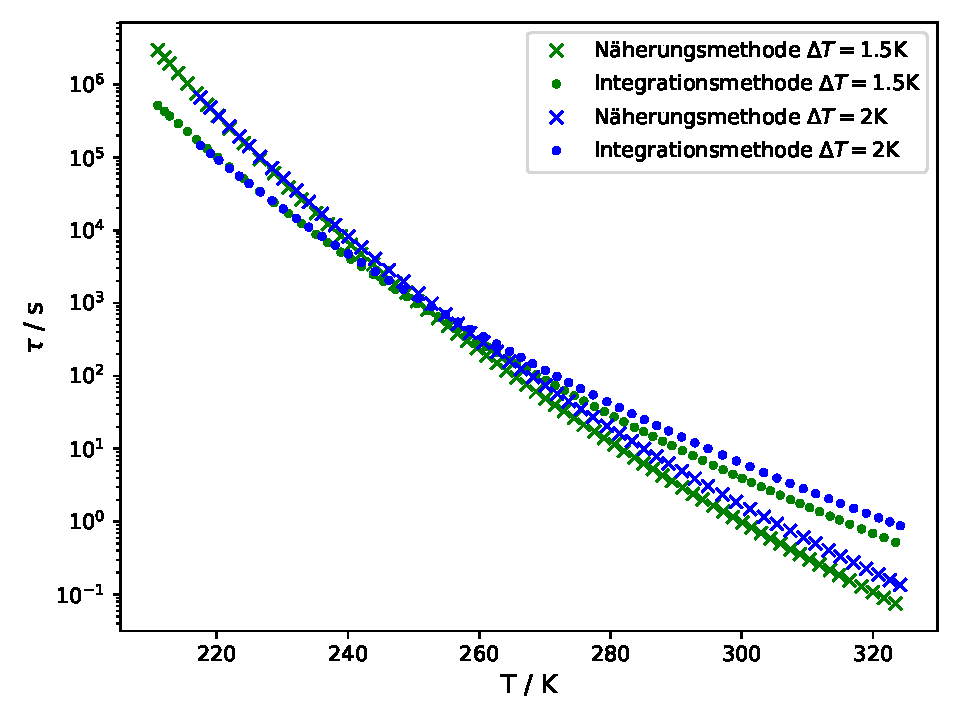
\includegraphics[width= \textwidth]{plots/tau_plot.pdf}
%    \caption{}
%    \label{fig:5}
%\end{figure}

